\section{Event Categorization}
\label{sec:Category}

\subsection{New MVA based categorization}
\todo{remove new, cite TMVA and BDT papers}
The VBF-enriched categories in Higgs coupling analysis focus more on VBF significance and the topology of final state to match the calculation in STXS framework, they are not suitable \todo{they're suitable but they're not optimal, rephrase} for this precise measurement of Higgs CP. For this reason a new 2 dimension boosted decision tree(BDT) is trained to have a high VBF purity signal region and reject both gluon-fusion and continuum \todo{$\gamma\gamma$} background events. Both of these two BDTs use 7 variables as input: $pT_{Hjj}$, $p_{Tt}$, $m_{jj}$, $\Delta\eta_{jj}$, $\delta\Phi_{\gamma\gamma, jj}$, $\eta^{Zepp}$, $\Delta R^{min}_{\gamma, j}$. They are trained independently with total\todo{what does total mean?}templates. Figure ~\ref{fig:ROC_ggh} ~\ref{fig:ROC_yy} show the trained BDT distribution and ROC curve, more details can be found in Appendix ~\ref{appendix:NewCate}
\todo{All details should be here, add plots of all the input variables between signal and background, add signal and background plots in all categories and OO bins after selection including dataside bands (take inspiration from ATL-COM-PHYS-2016-1784 plot 34 and 38, add a table with separation power of all variables used, add correlation matrices for the variables, all the parameters for the BDT (number of trees, depth ..etc)}
\begin{figure}[bp]
  \centering
  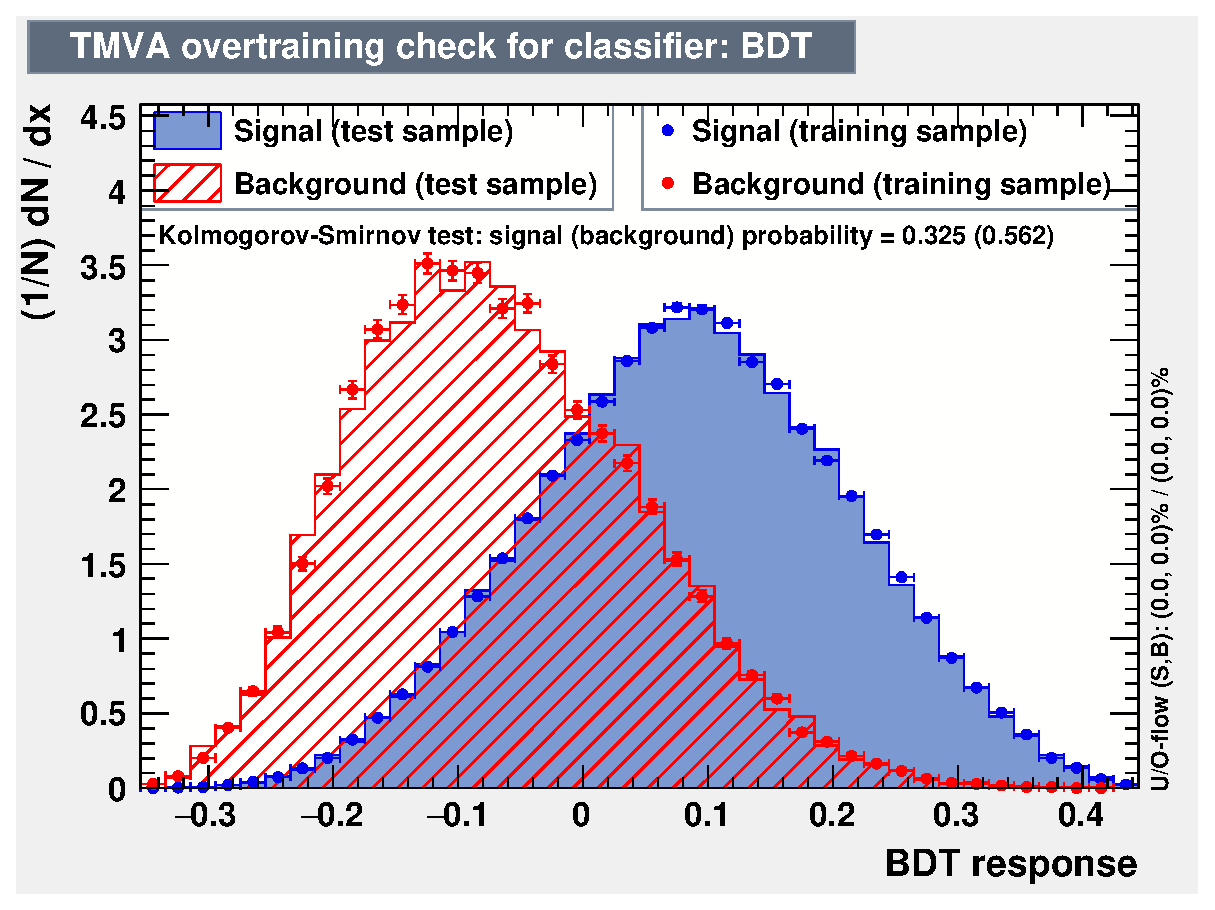
\includegraphics[width=0.45\linewidth]{figure/BDT/Perf_ggh/overtrain_BDT.eps}
  \includegraphics[width=0.45\linewidth]{figure/BDT/Perf_ggh/rejBvsS.eps}
  \caption{BDT distribution(left) and ROC curve(right) in VBF-ggF BDT training.}
  \label{fig:ROC_ggh}
\end{figure}

\begin{figure}[bp]
  \centering
  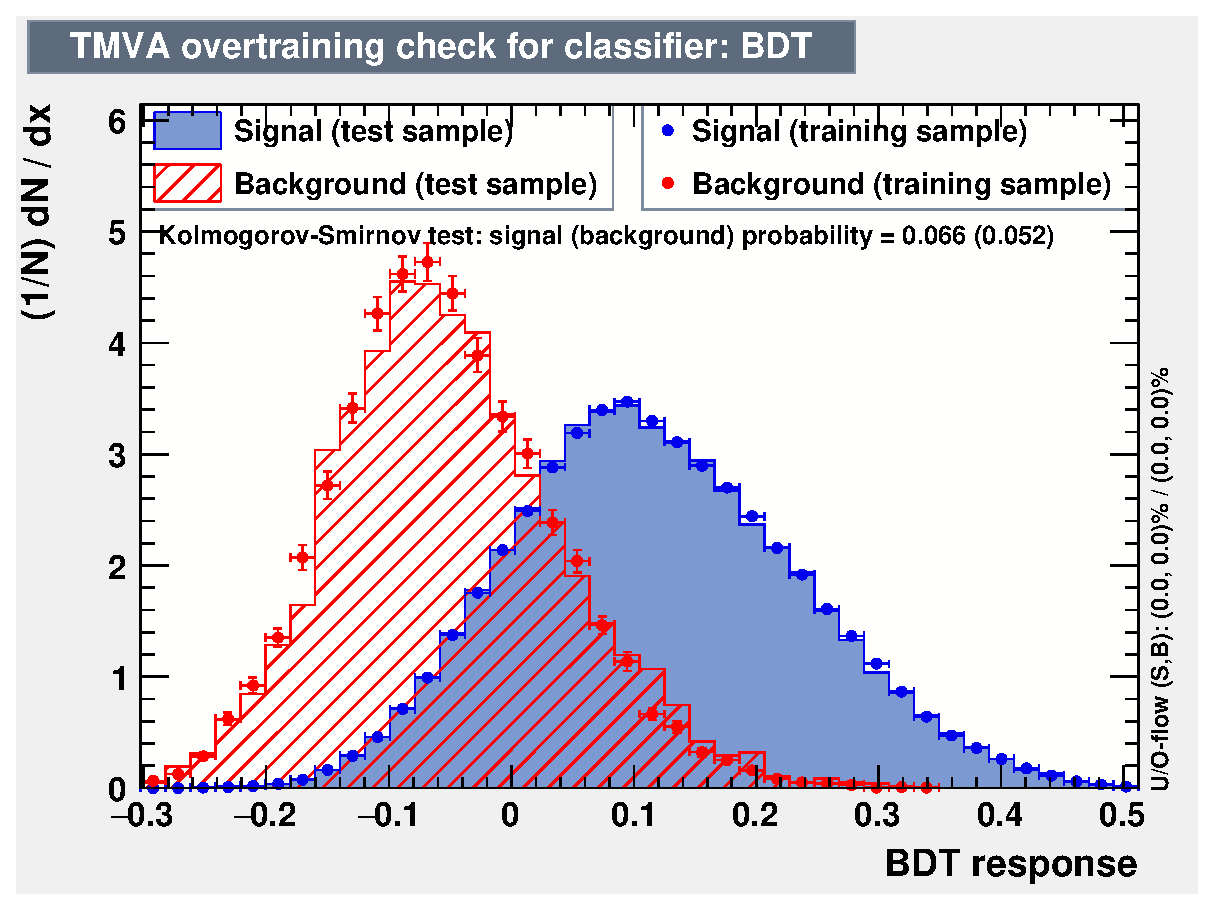
\includegraphics[width=0.45\linewidth]{figure/BDT/Perf_yy/overtrain_BDT.eps}
  \includegraphics[width=0.45\linewidth]{figure/BDT/Perf_yy/rejBvsS.eps}
  \caption{BDT distribution(left) and ROC curve(right) in VBF-$MC \gamma\gamma$ BDT training.}
  \label{fig:ROC_yy}
\end{figure}

The $BDT_{VBF/ggF}$ uses VBF purity $p= \frac{N_{VBF}}{N_{VBF}+N_{ggF}}$ as criterion. Since the maximum value of VBF purity appears at the edge of BDT range $BDT_{VBF/ggF}=1$, the working point is manually chosen to have the same VBF efficiency 34\% as in Higgs coupling categorizatio \todo{why is that?}. The VBF purity is increased from 87.7\% to 91.3\%, and gluon-fusion efficiency is decreased from 6.5\% to 4.5\%. \\

\begin{figure}[tbp]
  \centering
  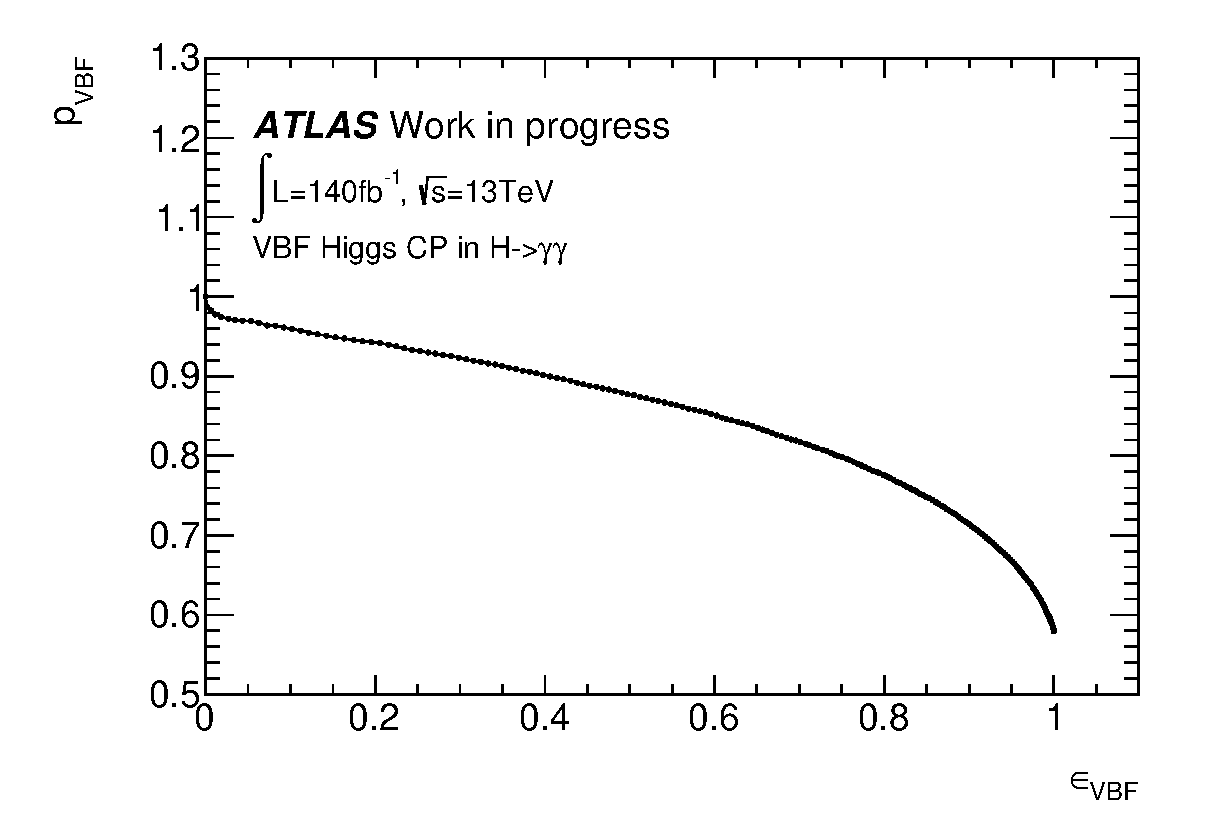
\includegraphics[width=0.45\linewidth]{figure/BDT/WP_vbfeff.eps}
  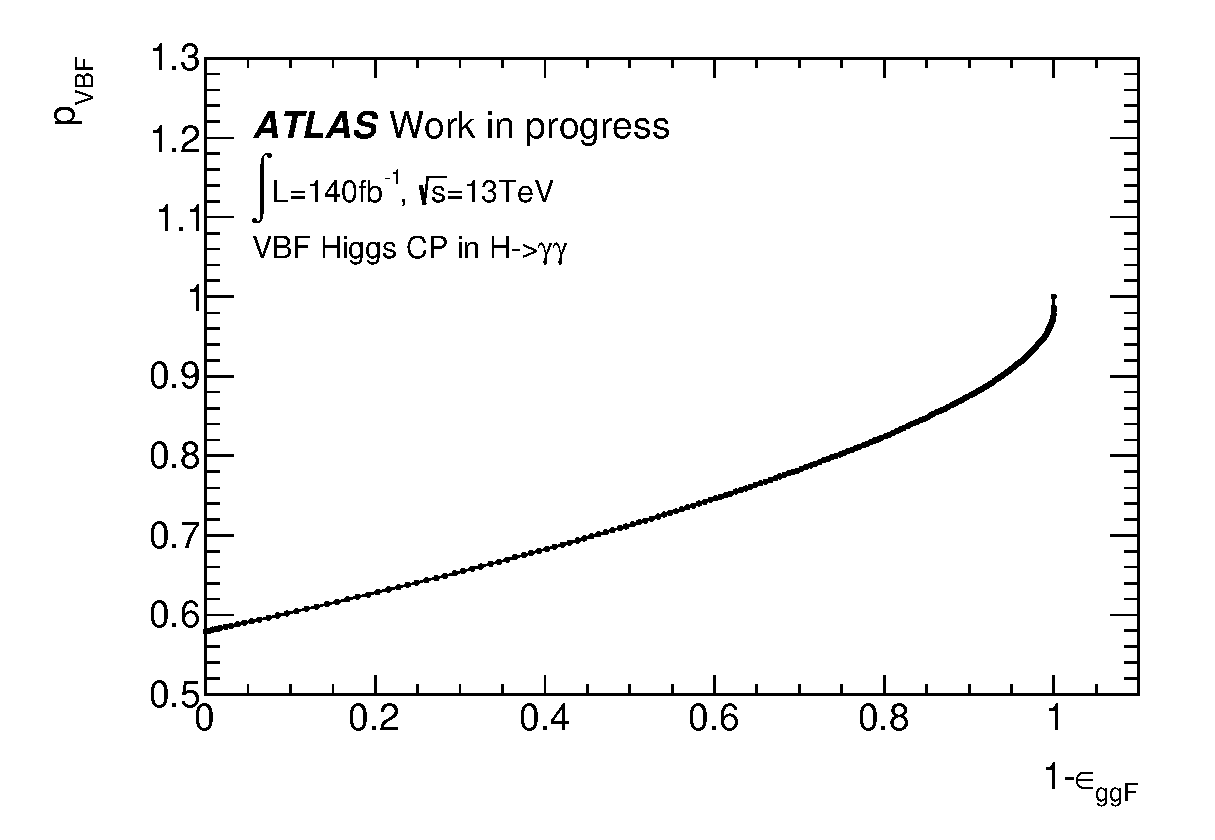
\includegraphics[width=0.45\linewidth]{figure/BDT/WP_ggfrej.eps}
  \caption{VBF purity with relationship of VBF efficiency(left) and ggF rejection(right). The working point is manually chosen with $\epsilon_{VBF}=34\%$, corresponding VBF purity and ggF rejection could be gotten.}
  \label{fig:vbfwp}
\end{figure}
\todo{explain the sudden dips/jumps in the plot}
Two regions are defined by the former criterion, naming \texttt{ggH\_tight} and \texttt{ggH\_loose} temporarily. Scanning $BDT_{VBF/\gamma\gamma}$ value in these two regions individually can provide a cut value at the global maximum VBF significance point. Figure ~\ref{fig:catedef} summary the definition of totally 4 categories, naming TT, TL, LT and LL. \\

\begin{figure}[tbp]
  \centering
  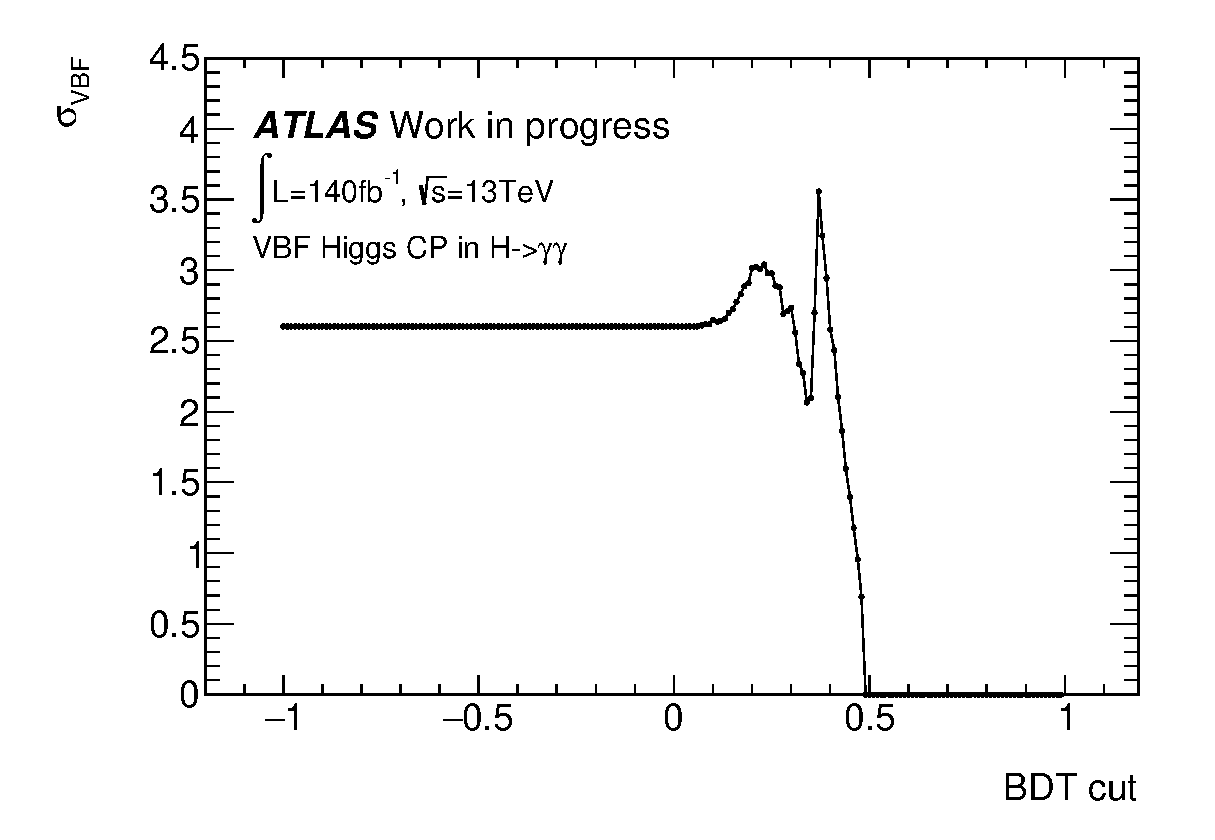
\includegraphics[width=0.45\linewidth]{figure/BDT/vbfsig_tight.eps}
  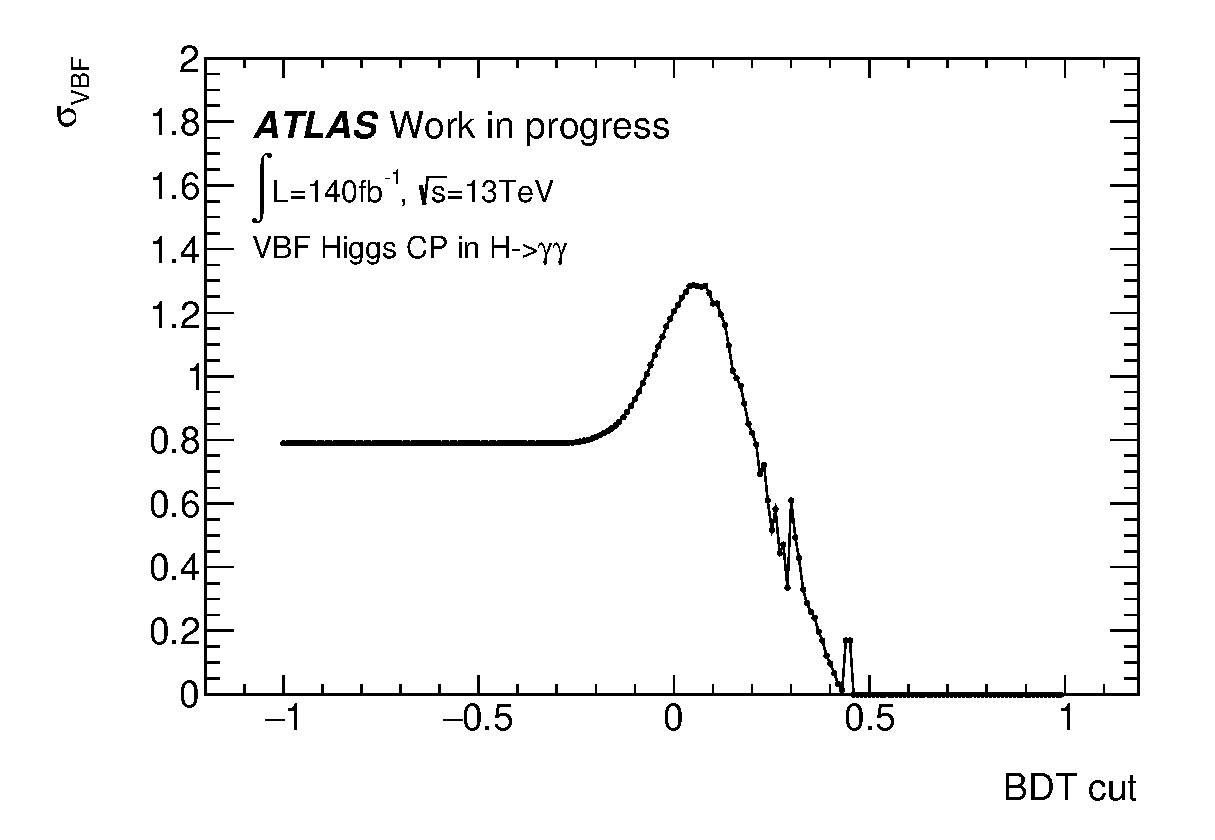
\includegraphics[width=0.45\linewidth]{figure/BDT/vbfsig_loose.eps}
  \caption{VBF significance in \texttt{ggH\_tight}(left) and \texttt{ggH\_loose}(right) regions with BDT cut value. In \texttt{ggH\_tight} the high fluctuation point has been ignored. }
  \label{fig:vbfsignificance}
\end{figure}

\begin{figure}[htbp]
  \centering
  \subfloat[]{
    \centering
    \includegraphics[width=.45\linewidth]{figure/BDT/NewCate.png}
  }
  \hfill
  \subfloat[]{
    \centering
    \begin{tabular}{ll}
      \toprule
      Category & Description \\
      \toprule
      TT       & $BDT_{VBF/ggF}>0.14, BDT_{VBF/\gamma\gamma}>0.23 $  \\
      TL       & $BDT_{VBF/ggF}>0.14, BDT_{VBF/\gamma\gamma}<0.23 $  \\
      LT       & $BDT_{VBF/ggF}<0.14, BDT_{VBF/\gamma\gamma}>0.05 $  \\
      LL       & $BDT_{VBF/ggF}<0.14, BDT_{VBF/\gamma\gamma}<0.05 $  \\
      \bottomrule
    \end{tabular}
  }
  \caption{The definition of 4 categories used in this analysis. }
  \label{fig:catedef}
\end{figure}

\begin{table}[htbp]
\centering
\begin{tabular}{|l|c|c|c|c|c|}
\hline
                  & TT    & TL     & LT      & LL       &  sum    \\ \hline
VBF               & 26.30 & 25.88  & 52.71   & 43.85    &  148.75 \\ \hline
ggF               & 1.72  & 3.22   & 24.06   & 81.77    &  110.76 \\ \hline
continuum         & 106   & 310    & 1886    & 16646    &  18949  \\ \hline
{[}120, 130{]}GeV & 21.25 & 62     & 377.25  & 3329.25  &  3789.7 \\ \hline
significance      & 5.49  & 3.20   & 2.63    & 0.75     &   \\ \hline
combined          & \multicolumn{4}{c|}{6.92}           &   \\ \hline
\end{tabular}
\label{tab:sigmaInCate}
\caption{Expectend event yields and VBF significance in 4 categories. Continuum background yield is normalized to sideband data, $[120, 130]GeV$ is estimated with background event number in full mass region times 0.2. VBF significance is calculated with background in mass window only.}
\end{table}



\subsection{Optimal observable binning}
\todo{add label for the section, use math style consistently everywhere}
The choice of optimal observable binning method can influence the sensitive of CP measurement. All events are divided into 6 positive-negative symmetry bins to ensure enough statistics and match the symmetry distribution of optimal observable \todo{use "trade-off" between purity and stats.}. With this restriction the binning can be decided by scanning only 2 parameter $p_1$ and $p_2$ with step 0.5 to have maximum global VBF significance:

%\begin{center}
%\begin{math}
$$
 Z_{\tilde{d}} = \sqrt(\Sigma_{i=0}^{6} Z_{i}^{2}) \\
 Z_{i} = Nvbf/\sqrt(Nvbf+Nggh+Nsr)
$$
%\end{math}
%\end{center}

With Nsr is the extrapolated background event number from sideband data. For different CP-mixing model the Z would be different, so in order to be model independent, an average Z value from d=-0.1 to 0.1 is chosen as the final criteria. Figure ~\ref{fig:Zvsp} shows the Z value for p1 and p2 scanning. The event number in every BDT categories and bins are shown in Table ~\ref{tab:Nevtinbins}
\todo{too short! what are the conclusions? haven't detailed how the edges where chosen}
\begin{figure}[tbp]
  \centering
  \includegraphics[width=0.45\linewidth]{figure/OObinning/binning.png}
  \includegraphics[width=0.45\linewidth]{figure/OObinning/Zscanning.png}
  \caption{The optimal observable binning is determined with 2 parameters. Global VBF significance is calculated in scanning two parameters with step of 0.5. ($p_1$, $p_2$) equal to (1, 2) and(1.5, 5,5) show very similar significance, while in order to get enough statistics in edge bins, the former one is chosen.}
  \label{fig:Zvsp}
\end{figure}

\begin{table}[htbp]
  \centering
  \subfloat[]{
  \begin{tabular}{l|ccccccc}
    VBF & {[}$-\infty$, -2{]}   & {[}-2, -1{]} & {[}-1, 0{]} & {[}0, 1{]} & {[}1, 2{]} & {[}2, $\infty${]} & sum   \\
    \toprule
    TT  & 6.29 & 3.63 & 3.22 & 3.20 & 3.63 & 6.32 & 26.30 \\ \hline
    TL  & 5.05 & 4.04 & 3.82 & 3.84 & 4.08 & 5.05 & 25.88 \\ \hline
    LT  & 8.96 & 7.72 & 9.78 & 9.65 & 7.70 & 8.90 & 52.71 \\ \hline
    LL  & 6.65 & 6.12 & 9.18 & 9.17 & 6.14 & 6.60 & 43.85 \\ 
    \bottomrule
  \end{tabular}
  }

  \subfloat[]{
  \begin{tabular}{l|ccccccc}
    ggF & {[}$-\infty$, -2{]}   & {[}-2, -1{]} & {[}-1, 0{]} & {[}0, 1{]} & {[}1, 2{]} & {[}2, $\infty${]} & sum   \\
    \toprule
    TT  & 0.28  & 0.23 & 0.33  & 0.32  & 0.26 & 0.29  & 1.72   \\ \hline
    TL  & 0.52  & 0.43 & 0.65  & 0.69  & 0.42 & 0.50  & 3.22   \\ \hline
    LT  & 3.95  & 2.76 & 5.23  & 5.31  & 2.79 & 4.02  & 24.06  \\ \hline
    LL  & 12.10 & 8.89 & 19.83 & 20.06 & 8.80 & 12.09 & 81.77  \\ 
    \bottomrule
  \end{tabular}
  }

  \subfloat[]{
  \begin{tabular}{l|ccccccc}
    Side-band data & {[}$-\infty$, -2{]}   & {[}-2, -1{]} & {[}-1, 0{]} & {[}0, 1{]} & {[}1, 2{]} & {[}2, $\infty${]} & sum   \\
    \toprule
    TT  & 18   & 13   & 13   & 12   & 13   & 16   & 85    \\ \hline
    TL  & 48   & 39   & 41   & 39   & 40   & 41   & 248   \\ \hline
    LT  & 216  & 203  & 329  & 325  & 214  & 222  & 1509  \\ \hline
    LL  & 2303 & 1539 & 2837 & 2702 & 1587 & 2349 & 13317 \\
    \bottomrule
  \end{tabular}
  }

  \label{tab:Nevtinbins}
  \caption{Expected signal event yield and sideband data number in each bins and categories. }
\end{table}

